% Options for packages loaded elsewhere
\PassOptionsToPackage{unicode}{hyperref}
\PassOptionsToPackage{hyphens}{url}
\PassOptionsToPackage{dvipsnames,svgnames,x11names}{xcolor}
%
\documentclass[
  letterpaper,
  DIV=11,
  numbers=noendperiod]{scrreprt}

\usepackage{amsmath,amssymb}
\usepackage{iftex}
\ifPDFTeX
  \usepackage[T1]{fontenc}
  \usepackage[utf8]{inputenc}
  \usepackage{textcomp} % provide euro and other symbols
\else % if luatex or xetex
  \usepackage{unicode-math}
  \defaultfontfeatures{Scale=MatchLowercase}
  \defaultfontfeatures[\rmfamily]{Ligatures=TeX,Scale=1}
\fi
\usepackage{lmodern}
\ifPDFTeX\else  
    % xetex/luatex font selection
\fi
% Use upquote if available, for straight quotes in verbatim environments
\IfFileExists{upquote.sty}{\usepackage{upquote}}{}
\IfFileExists{microtype.sty}{% use microtype if available
  \usepackage[]{microtype}
  \UseMicrotypeSet[protrusion]{basicmath} % disable protrusion for tt fonts
}{}
\makeatletter
\@ifundefined{KOMAClassName}{% if non-KOMA class
  \IfFileExists{parskip.sty}{%
    \usepackage{parskip}
  }{% else
    \setlength{\parindent}{0pt}
    \setlength{\parskip}{6pt plus 2pt minus 1pt}}
}{% if KOMA class
  \KOMAoptions{parskip=half}}
\makeatother
\usepackage{xcolor}
\setlength{\emergencystretch}{3em} % prevent overfull lines
\setcounter{secnumdepth}{-\maxdimen} % remove section numbering
% Make \paragraph and \subparagraph free-standing
\makeatletter
\ifx\paragraph\undefined\else
  \let\oldparagraph\paragraph
  \renewcommand{\paragraph}{
    \@ifstar
      \xxxParagraphStar
      \xxxParagraphNoStar
  }
  \newcommand{\xxxParagraphStar}[1]{\oldparagraph*{#1}\mbox{}}
  \newcommand{\xxxParagraphNoStar}[1]{\oldparagraph{#1}\mbox{}}
\fi
\ifx\subparagraph\undefined\else
  \let\oldsubparagraph\subparagraph
  \renewcommand{\subparagraph}{
    \@ifstar
      \xxxSubParagraphStar
      \xxxSubParagraphNoStar
  }
  \newcommand{\xxxSubParagraphStar}[1]{\oldsubparagraph*{#1}\mbox{}}
  \newcommand{\xxxSubParagraphNoStar}[1]{\oldsubparagraph{#1}\mbox{}}
\fi
\makeatother

\usepackage{color}
\usepackage{fancyvrb}
\newcommand{\VerbBar}{|}
\newcommand{\VERB}{\Verb[commandchars=\\\{\}]}
\DefineVerbatimEnvironment{Highlighting}{Verbatim}{commandchars=\\\{\}}
% Add ',fontsize=\small' for more characters per line
\usepackage{framed}
\definecolor{shadecolor}{RGB}{241,243,245}
\newenvironment{Shaded}{\begin{snugshade}}{\end{snugshade}}
\newcommand{\AlertTok}[1]{\textcolor[rgb]{0.68,0.00,0.00}{#1}}
\newcommand{\AnnotationTok}[1]{\textcolor[rgb]{0.37,0.37,0.37}{#1}}
\newcommand{\AttributeTok}[1]{\textcolor[rgb]{0.40,0.45,0.13}{#1}}
\newcommand{\BaseNTok}[1]{\textcolor[rgb]{0.68,0.00,0.00}{#1}}
\newcommand{\BuiltInTok}[1]{\textcolor[rgb]{0.00,0.23,0.31}{#1}}
\newcommand{\CharTok}[1]{\textcolor[rgb]{0.13,0.47,0.30}{#1}}
\newcommand{\CommentTok}[1]{\textcolor[rgb]{0.37,0.37,0.37}{#1}}
\newcommand{\CommentVarTok}[1]{\textcolor[rgb]{0.37,0.37,0.37}{\textit{#1}}}
\newcommand{\ConstantTok}[1]{\textcolor[rgb]{0.56,0.35,0.01}{#1}}
\newcommand{\ControlFlowTok}[1]{\textcolor[rgb]{0.00,0.23,0.31}{\textbf{#1}}}
\newcommand{\DataTypeTok}[1]{\textcolor[rgb]{0.68,0.00,0.00}{#1}}
\newcommand{\DecValTok}[1]{\textcolor[rgb]{0.68,0.00,0.00}{#1}}
\newcommand{\DocumentationTok}[1]{\textcolor[rgb]{0.37,0.37,0.37}{\textit{#1}}}
\newcommand{\ErrorTok}[1]{\textcolor[rgb]{0.68,0.00,0.00}{#1}}
\newcommand{\ExtensionTok}[1]{\textcolor[rgb]{0.00,0.23,0.31}{#1}}
\newcommand{\FloatTok}[1]{\textcolor[rgb]{0.68,0.00,0.00}{#1}}
\newcommand{\FunctionTok}[1]{\textcolor[rgb]{0.28,0.35,0.67}{#1}}
\newcommand{\ImportTok}[1]{\textcolor[rgb]{0.00,0.46,0.62}{#1}}
\newcommand{\InformationTok}[1]{\textcolor[rgb]{0.37,0.37,0.37}{#1}}
\newcommand{\KeywordTok}[1]{\textcolor[rgb]{0.00,0.23,0.31}{\textbf{#1}}}
\newcommand{\NormalTok}[1]{\textcolor[rgb]{0.00,0.23,0.31}{#1}}
\newcommand{\OperatorTok}[1]{\textcolor[rgb]{0.37,0.37,0.37}{#1}}
\newcommand{\OtherTok}[1]{\textcolor[rgb]{0.00,0.23,0.31}{#1}}
\newcommand{\PreprocessorTok}[1]{\textcolor[rgb]{0.68,0.00,0.00}{#1}}
\newcommand{\RegionMarkerTok}[1]{\textcolor[rgb]{0.00,0.23,0.31}{#1}}
\newcommand{\SpecialCharTok}[1]{\textcolor[rgb]{0.37,0.37,0.37}{#1}}
\newcommand{\SpecialStringTok}[1]{\textcolor[rgb]{0.13,0.47,0.30}{#1}}
\newcommand{\StringTok}[1]{\textcolor[rgb]{0.13,0.47,0.30}{#1}}
\newcommand{\VariableTok}[1]{\textcolor[rgb]{0.07,0.07,0.07}{#1}}
\newcommand{\VerbatimStringTok}[1]{\textcolor[rgb]{0.13,0.47,0.30}{#1}}
\newcommand{\WarningTok}[1]{\textcolor[rgb]{0.37,0.37,0.37}{\textit{#1}}}

\providecommand{\tightlist}{%
  \setlength{\itemsep}{0pt}\setlength{\parskip}{0pt}}\usepackage{longtable,booktabs,array}
\usepackage{calc} % for calculating minipage widths
% Correct order of tables after \paragraph or \subparagraph
\usepackage{etoolbox}
\makeatletter
\patchcmd\longtable{\par}{\if@noskipsec\mbox{}\fi\par}{}{}
\makeatother
% Allow footnotes in longtable head/foot
\IfFileExists{footnotehyper.sty}{\usepackage{footnotehyper}}{\usepackage{footnote}}
\makesavenoteenv{longtable}
\usepackage{graphicx}
\makeatletter
\newsavebox\pandoc@box
\newcommand*\pandocbounded[1]{% scales image to fit in text height/width
  \sbox\pandoc@box{#1}%
  \Gscale@div\@tempa{\textheight}{\dimexpr\ht\pandoc@box+\dp\pandoc@box\relax}%
  \Gscale@div\@tempb{\linewidth}{\wd\pandoc@box}%
  \ifdim\@tempb\p@<\@tempa\p@\let\@tempa\@tempb\fi% select the smaller of both
  \ifdim\@tempa\p@<\p@\scalebox{\@tempa}{\usebox\pandoc@box}%
  \else\usebox{\pandoc@box}%
  \fi%
}
% Set default figure placement to htbp
\def\fps@figure{htbp}
\makeatother
% definitions for citeproc citations
\NewDocumentCommand\citeproctext{}{}
\NewDocumentCommand\citeproc{mm}{%
  \begingroup\def\citeproctext{#2}\cite{#1}\endgroup}
\makeatletter
 % allow citations to break across lines
 \let\@cite@ofmt\@firstofone
 % avoid brackets around text for \cite:
 \def\@biblabel#1{}
 \def\@cite#1#2{{#1\if@tempswa , #2\fi}}
\makeatother
\newlength{\cslhangindent}
\setlength{\cslhangindent}{1.5em}
\newlength{\csllabelwidth}
\setlength{\csllabelwidth}{3em}
\newenvironment{CSLReferences}[2] % #1 hanging-indent, #2 entry-spacing
 {\begin{list}{}{%
  \setlength{\itemindent}{0pt}
  \setlength{\leftmargin}{0pt}
  \setlength{\parsep}{0pt}
  % turn on hanging indent if param 1 is 1
  \ifodd #1
   \setlength{\leftmargin}{\cslhangindent}
   \setlength{\itemindent}{-1\cslhangindent}
  \fi
  % set entry spacing
  \setlength{\itemsep}{#2\baselineskip}}}
 {\end{list}}
\usepackage{calc}
\newcommand{\CSLBlock}[1]{\hfill\break\parbox[t]{\linewidth}{\strut\ignorespaces#1\strut}}
\newcommand{\CSLLeftMargin}[1]{\parbox[t]{\csllabelwidth}{\strut#1\strut}}
\newcommand{\CSLRightInline}[1]{\parbox[t]{\linewidth - \csllabelwidth}{\strut#1\strut}}
\newcommand{\CSLIndent}[1]{\hspace{\cslhangindent}#1}

\KOMAoption{captions}{tableheading}
\makeatletter
\@ifpackageloaded{bookmark}{}{\usepackage{bookmark}}
\makeatother
\makeatletter
\@ifpackageloaded{caption}{}{\usepackage{caption}}
\AtBeginDocument{%
\ifdefined\contentsname
  \renewcommand*\contentsname{Table of contents}
\else
  \newcommand\contentsname{Table of contents}
\fi
\ifdefined\listfigurename
  \renewcommand*\listfigurename{List of Figures}
\else
  \newcommand\listfigurename{List of Figures}
\fi
\ifdefined\listtablename
  \renewcommand*\listtablename{List of Tables}
\else
  \newcommand\listtablename{List of Tables}
\fi
\ifdefined\figurename
  \renewcommand*\figurename{Figure}
\else
  \newcommand\figurename{Figure}
\fi
\ifdefined\tablename
  \renewcommand*\tablename{Table}
\else
  \newcommand\tablename{Table}
\fi
}
\@ifpackageloaded{float}{}{\usepackage{float}}
\floatstyle{ruled}
\@ifundefined{c@chapter}{\newfloat{codelisting}{h}{lop}}{\newfloat{codelisting}{h}{lop}[chapter]}
\floatname{codelisting}{Listing}
\newcommand*\listoflistings{\listof{codelisting}{List of Listings}}
\makeatother
\makeatletter
\makeatother
\makeatletter
\@ifpackageloaded{caption}{}{\usepackage{caption}}
\@ifpackageloaded{subcaption}{}{\usepackage{subcaption}}
\makeatother

\usepackage{bookmark}

\IfFileExists{xurl.sty}{\usepackage{xurl}}{} % add URL line breaks if available
\urlstyle{same} % disable monospaced font for URLs
\hypersetup{
  colorlinks=true,
  linkcolor={blue},
  filecolor={Maroon},
  citecolor={Blue},
  urlcolor={Blue},
  pdfcreator={LaTeX via pandoc}}


\author{}
\date{}

\begin{document}

\renewcommand*\contentsname{Table of contents}
{
\hypersetup{linkcolor=}
\setcounter{tocdepth}{2}
\tableofcontents
}

\bookmarksetup{startatroot}

\chapter*{National Park Service Yellow-billed Loons Monitoring Data
Management
Procedures}\label{national-park-service-yellow-billed-loons-monitoring-data-management-procedures}
\addcontentsline{toc}{chapter}{National Park Service Yellow-billed Loons
Monitoring Data Management Procedures}

\markboth{National Park Service Yellow-billed Loons Monitoring Data
Management Procedures}{National Park Service Yellow-billed Loons
Monitoring Data Management Procedures}

Scott D. Miller\\
Information Technology Specialist\\
U.S. Department of the Interior\\
240 W. 5th Ave.\\
Anchorage, AK 99501

This book contains data management procedures for the National Park
Service's Yellow-billed loons monitoring program in Bering Land Bridge
National Preserve and Cape Krusenstern National Monument, Alaska.

See Flamme and Miller (2018) for the monitoring protocol.

\bookmarksetup{startatroot}

\chapter{Data ownership and
sensitivity}\label{data-ownership-and-sensitivity}

Data collected by the National Park Service, with limited exceptions are
in the public domain:

\emph{Data and content created by government employees within the scope
of their employment are not subject to domestic copyright protection
under 17 U.S.C. 105. Government works are by default in the U.S. Public
Domain.}

Portions of the Yellow-billed and Red-throated loons monitoring data
containing spatial locations of loons and nests are considered sensitive
data by the National Park Service, and are not to be shared with the
general public.

\emph{Under National Parks Omnibus Management Act, Section 207, of 16
U.S.C. § 5937; Specific location (geographic coordinates) of this
species of concern will not be released to the general public due to
their global rarity and nest site fidelity. Any such data collected will
be redacted from the publicly released datasets. This protects
collaborating agencies data as well; but does not preclude sharing
between collaborating agencies. Processed data with coordinates redacted
(such as summaries, processed maps, or products) remain publicly
available. This will be done indefinitely (}(Koelsch 2019)\emph{).}

Data not considered sensitive, such as plot locations, lake perimeters,
data summaries and secondary datasets not prohibited by the above
restrictions are to be distributed freely as U.S. Public Works.

\bookmarksetup{startatroot}

\chapter*{Deliverables Schedule}\label{deliverables-schedule}
\addcontentsline{toc}{chapter}{Deliverables Schedule}

\markboth{Deliverables Schedule}{Deliverables Schedule}

The National Park Service's Western Yellow-billed Loons monitoring
program will collect and maintain the following data deliverables. Each
mandatory deliverable should be fulfilled during a survey and delivered
to the ARCN data manager for integration with the master loons
monitoring SQL Server database and the
\href{https://irma.nps.gov/DataStore/Reference/Profile/2216938}{NPS Data
Store}.

\begin{longtable}[]{@{}ll@{}}
\toprule\noalign{}
Identifier & Deliverable \\
\midrule\noalign{}
\endhead
\bottomrule\noalign{}
\endlastfoot
YB01 & Survey geodatabase (YBLO.gdb) \\
YB02 & Park Observer files \\
YB03 & Waypoints \\
YB04 & Data collection forms, booklets and field notebooks \\
YB05 & Deprecated \\
YB06 & Observations data file \\
YB07 & Tracklogs \\
YB08 & Lakes dataset \\
YB09 & Plots dataset \\
YB10 & Deprecated \\
YB11 & Photographs \\
YB12 & Data processing scripts \\
\end{longtable}

\bookmarksetup{startatroot}

\chapter*{YB01: Survey geodatabase
(YBLO.gdb)}\label{yb01-survey-geodatabase-yblo.gdb}
\addcontentsline{toc}{chapter}{YB01: Survey geodatabase (YBLO.gdb)}

\markboth{YB01: Survey geodatabase (YBLO.gdb)}{YB01: Survey geodatabase
(YBLO.gdb)}

\emph{Format:} Geospatial layer

\emph{Schedule:} Remeasurement + 1 year

\emph{Responsibility:} PI*

\emph{Description:} Geodatabase containing processed QA/QC-checked
survey data, including feature classes/layers of the loon and nest data.
There is a different geodatabase for each year.

\emph{Specifications:} Compressed .zip archive containing the
geodatabase.

\emph{FileNamingScheme:} Deliverable YB01 should be named {[}YB01' YYYY
Loon Survey Survey geodatabase.zip {]} where YYYY represents the integer
year of the survey.

\bookmarksetup{startatroot}

\chapter*{YB02: Park Observer files}\label{yb02-park-observer-files}
\addcontentsline{toc}{chapter}{YB02: Park Observer files}

\markboth{YB02: Park Observer files}{YB02: Park Observer files}

\emph{Format:} .poz and/or comma separated values (CSV) text files.

\emph{Schedule:} Remeasurement + 1 year

\emph{Responsibility:} PI, DM

\emph{Description:} Compressed .zip archive containing iPad Park
Observer .pov files and affiliated geodatabase containing the raw, field
collected data prior to importing and processing those data in the GIS.

\emph{Specifications:} Park Observer files in compressed (.zip) format.
Human and machine readable text format (JSON, CSV, or other).

\emph{FileNamingScheme:} Deliverable YB02 should be named {[}YB02' YYYY
Loon Survey Park Observer files.zip{]} where YYYY represents the integer
year of the survey.

\bookmarksetup{startatroot}

\chapter*{YB03: Waypoints}\label{yb03-waypoints}
\addcontentsline{toc}{chapter}{YB03: Waypoints}

\markboth{YB03: Waypoints}{YB03: Waypoints}

\emph{Format:} Human and machine readable text file format.

\emph{Schedule:} Remeasurement + 1 year

\emph{Responsibility:} PI

\emph{Description:} Waypoints collected by the pilot or observer during
a loon survey

\emph{Specifications:} Human and machine readable text format (JSON,
CSV, or other).

\emph{FileNamingScheme:} Deliverable YB03 should be named {[}YB03' YYYY
Loon Survey Waypoints{]} where YYYY represents the integer year of the
survey.

\bookmarksetup{startatroot}

\chapter*{YB04: Data collection forms, booklets and field
notebooks}\label{yb04-data-collection-forms-booklets-and-field-notebooks}
\addcontentsline{toc}{chapter}{YB04: Data collection forms, booklets and
field notebooks}

\markboth{YB04: Data collection forms, booklets and field
notebooks}{YB04: Data collection forms, booklets and field notebooks}

\emph{Format:} Physical forms and TIFF or PDF scans

\emph{Schedule:} Remeasurement + 1 year

\emph{Responsibility:} PI

\emph{Description:} Deliverable YB04 consists of physical paper data
collection forms, if applicable.

\emph{Specifications:} Legible paper printouts.

\emph{FileNamingScheme:} Deliverable YB04 should be named {[}YB04' YYYY
Loon Survey Data collection forms, booklets and field notebooks{]} where
YYYY represents the integer year of the survey.

\bookmarksetup{startatroot}

\chapter*{YB05: Deprecated}\label{yb05-deprecated}
\addcontentsline{toc}{chapter}{YB05: Deprecated}

\markboth{YB05: Deprecated}{YB05: Deprecated}

\emph{Format:} NA

\emph{Schedule:} NA

\emph{Responsibility:} NA

\emph{Description:} NA

\emph{Specifications:} NA

\emph{FileNamingScheme:} NA

\bookmarksetup{startatroot}

\chapter*{YB06: Observations data
file}\label{yb06-observations-data-file}
\addcontentsline{toc}{chapter}{YB06: Observations data file}

\markboth{YB06: Observations data file}{YB06: Observations data file}

\emph{Format:} Comma separated values(CSV) text file.

\emph{Schedule:} Remeasurement + 1 year

\emph{Responsibility:} PI

\emph{Description:} Deliverable YB06 consists of the digitized loons
data collected during a survey. These data should be in comma separated
values text file format.

\emph{Specifications:} Human and machine readable text format (JSON,
CSV, or other).

\emph{FileNamingScheme:} Deliverable YB06 should be named {[}YB06' YYYY
Loon Survey Observations data file{]} where YYYY represents the integer
year of the survey.

\bookmarksetup{startatroot}

\chapter*{YB07: Tracklogs}\label{yb07-tracklogs}
\addcontentsline{toc}{chapter}{YB07: Tracklogs}

\markboth{YB07: Tracklogs}{YB07: Tracklogs}

\emph{Format:} Human and machine readable text file format.

\emph{Schedule:} Remeasurement + 1 year

\emph{Responsibility:} PI

\emph{Description:} Deliverable YB07 consists of the digitized tracklog
data collected during a survey. These data should be in comma separated
values text file format.

\emph{Specifications:} Human and machine readable text format (JSON,
CSV, or other).

\emph{FileNamingScheme:} Deliverable YB07 should be named {[}YB07' YYYY
Loon Survey Tracklogs{]} where YYYY represents the integer year of the
survey.

\bookmarksetup{startatroot}

\chapter*{YB08: Lakes dataset}\label{yb08-lakes-dataset}
\addcontentsline{toc}{chapter}{YB08: Lakes dataset}

\markboth{YB08: Lakes dataset}{YB08: Lakes dataset}

\emph{Format:} Human and machine readable text file format.

\emph{Schedule:} Remeasurement + 1 year

\emph{Responsibility:} PI

\emph{Description:} Deliverable YB08 consists of a spatial data file
containing the surveyed lakes polygons. These data should be in comma
separated values text file format.

\emph{Specifications:} Human and machine readable text format (JSON,
CSV, or other).

\emph{FileNamingScheme:} Deliverable YB08 should be named {[}YB08' YYYY
Loon Survey Lakes dataset{]} where YYYY represents the integer year of
the survey.

\bookmarksetup{startatroot}

\chapter*{YB09: Plots dataset}\label{yb09-plots-dataset}
\addcontentsline{toc}{chapter}{YB09: Plots dataset}

\markboth{YB09: Plots dataset}{YB09: Plots dataset}

\emph{Format:} Human and machine readable text file format.

\emph{Schedule:} Remeasurement + 1 year

\emph{Responsibility:} PI

\emph{Description:} Deliverable YB09 consists of a spatial data file
containing the surveyed Plot polygons. These data should be in comma
separated values text file format.

\emph{Specifications:} Human and machine readable text format (JSON,
CSV, or other).

\emph{FileNamingScheme:} Deliverable YB09 should be named {[}YB09' YYYY
Loon Survey Plots dataset{]} where YYYY represents the integer year of
the survey.

\bookmarksetup{startatroot}

\chapter*{YB10: Deprecated}\label{yb10-deprecated}
\addcontentsline{toc}{chapter}{YB10: Deprecated}

\markboth{YB10: Deprecated}{YB10: Deprecated}

\emph{Format:} NA

\emph{Schedule:} NA

\emph{Responsibility:} NA

\emph{Description:} NA

\emph{Specifications:} NA

\emph{FileNamingScheme:} NA

\bookmarksetup{startatroot}

\chapter*{YB11: Photographs}\label{yb11-photographs}
\addcontentsline{toc}{chapter}{YB11: Photographs}

\markboth{YB11: Photographs}{YB11: Photographs}

\emph{Format:} Tag Image File (\emph{.TIF, }.TIFF) is preferable. Joint
Photographic Experts Group (\emph{.JPEG, }.JPG) is acceptable.

\emph{Schedule:} Remeasurement + 1 year

\emph{Responsibility:} PI

\emph{Description:} Deliverable YB11 consists of photographs taken
during a survey.

\emph{Specifications:} Tag Image File Format.

\emph{FileNamingScheme:} Deliverable YB11 should be named {[}YB11' YYYY
Loon Survey Photographs{]} where YYYY represents the integer year of the
survey.

\bookmarksetup{startatroot}

\chapter*{YB12: Data processing
scripts}\label{yb12-data-processing-scripts}
\addcontentsline{toc}{chapter}{YB12: Data processing scripts}

\markboth{YB12: Data processing scripts}{YB12: Data processing scripts}

\emph{Format:} NA

\emph{Schedule:} NA

\emph{Responsibility:} NA

\emph{Description:} Deliverable YB12 consists of data processing
scripts, database procedures, etc, that are used to cleanse, develop and
certify the survey data products.

\emph{Specifications:} Well documented.

\emph{FileNamingScheme:} Deliverable YB12 should be named {[}YB12' YYYY
Loon Survey Data processing scripts{]} where YYYY represents the integer
year of the survey.

\bookmarksetup{startatroot}

\chapter{Data Management Lifecycle And
Procedures}\label{data-management-lifecycle-and-procedures}

The YBLO monitoring team recognizes the importance of following a
fastidious and disciplined data management life cycle to promote data
longevity and informational quality over an anticipated term of decades.

This section covers the data management life cycle for the Yellow-billed
loons monitoring program after data is collected. For field data
collection procedures and methods follow the standard operating
procedures in (Flamme and Miller (2018)) available from the
\href{https://irma.nps.gov/DataStore/Reference/Profile/2216938}{Yellow-billed
loons Project Reference} in the NPS Data Store.

\section{Collect data according to the YBLO standard operating
procedures}\label{collect-data-according-to-the-yblo-standard-operating-procedures}

Follow the data collection SOPs in the loons monitoring protocol and
SOPs at \url{https://irma.nps.gov/DataStore/Reference/Profile/2216938}

\section{Organize and re-name raw data deliverable
files}\label{organize-and-re-name-raw-data-deliverable-files}

Upon returning from a field survey the first task is to organize and
re-name raw field data deliverables in the loons monitoring shared
directory
(\texttt{O:\textbackslash{}Monitoring\textbackslash{}Vital\ Signs\textbackslash{}Yellow-billed\ Loons\textbackslash{}Data}).
Figure 1 shows an example of a well organized data directory.

File organization and naming procedures are in the
\href{DeliverablesSchedule.html}{Deliverables Schedule} and personnel
are expected to follow them closely. Doing so will assure future users
know what is what, and will aid in backtracking data processing
procedures if errors are discovered. Our goal is reproducibility and the
highest data quality possible. Look over the Deliverables Schedule
and/or familiarize yourself with how the previous year's data files are
named and organized in the loons monitoring files directory. These file
names are recorded in the database so that users can back-track,
following a chain of processing steps to raw deliverable files if
problems are encountered in the future.

\pandocbounded{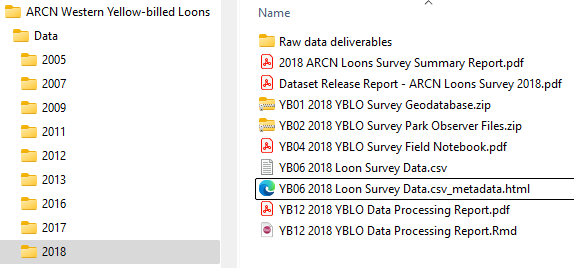
\includegraphics[keepaspectratio]{images/clipboard-979262005.png}}

Figure 1. A well organized loon survey data deliverables directory. Raw
data files are separate from final, processed deliverables. Filenames
are tagged with their deliverable identifiers. Data processing and
quality control scripts and summaries are included.

\section{Process the deliverables for quality and logical
consistency}\label{process-the-deliverables-for-quality-and-logical-consistency}

There are no specific procedures for processing data quality, other than
the suggestion to use a reproducible science platform such as R Markdown
or Quarto, Python/Jupyter notebooks, etc. to document the procedures you
undertook and data sources you used.

Putting effort into creating tidy data will make all the following data
processing procedures easier. If you are not familiar with the concept
of tidy data then please read Wickham (2014) (a fantastic, quick read
that will make your life as a scientist much easier).

Look in prior year's data directories at data processing scripts
prefixed with `YB12' to see how data were processed for quality and
database integration.

Look for:

\begin{itemize}
\item
  Missing or erroneous spatial coordinates
\item
  Missing or impossible Plot numbers
\item
  Incidental (non-Plot) observations
\item
  Extraneous (non-protocol mandated) wildlife sightings
\item
  Consistent and standard species codes
\item
  Missing counts, nest, pair or other poor quality records
\item
  Validate the data against a report, if available
\end{itemize}

Data processing scripts are a deliverable (YB12) and should be saved in
the survey's data directory and name similar to `YB12 YYYY Loon Survey
DESCRIPTION.ext'. Example:
\texttt{YB12\ 2023\ Loon\ Survey\ Data\ Processing\ Script.rmd}.

\section{Integrate the deliverables with the master loons monitoring
database}\label{integrate-the-deliverables-with-the-master-loons-monitoring-database}

Once the loon observations, lakes, plots and other files are processed
you enter them into the loons monitoring SQL Server database. There are
many methods to transfer data from deliverable files into a database.
SQL Server Management Studio has a data import/export wizard. R and
Python have packages and methods for moving data. You could also use
Excel formulas to generate a series of INSERT queries. Data from 2005 -
2023 were moved via R scripts. Look for those scripts, prefixed with
`YB12' in the loons directories or References in Data Store. Modify the
scripts as needed.

One easy way is to shape the dataset that is to be imported into the
database such that each column is named exactly the same as the schema
of the database's SurveyData table. Then you can generate a script of
SQL INSERT queries using this function:

\begin{Shaded}
\begin{Highlighting}[]
\CommentTok{\# Function to convert a data frame into SQL INSERT queries}
\NormalTok{DataFrameToSQLInsertQueries }\OtherTok{\textless{}{-}} \ControlFlowTok{function}\NormalTok{(SourceDataFrame, DestinationTableName) \{}
  
  \CommentTok{\# Helper: convert a single value to SQL literal}
\NormalTok{  ToSQLValue }\OtherTok{\textless{}{-}} \ControlFlowTok{function}\NormalTok{(x) \{}
    \ControlFlowTok{if}\NormalTok{ (}\FunctionTok{is.na}\NormalTok{(x)) \{}
      \FunctionTok{return}\NormalTok{(}\StringTok{"NULL"}\NormalTok{)}
\NormalTok{    \}}
    
    \ControlFlowTok{if}\NormalTok{ (}\FunctionTok{trimws}\NormalTok{(x) }\SpecialCharTok{==} \StringTok{\textquotesingle{}\textquotesingle{}}\NormalTok{) \{}
      \FunctionTok{return}\NormalTok{(}\StringTok{"NULL"}\NormalTok{)}
\NormalTok{    \}}
    
    \ControlFlowTok{if}\NormalTok{ (}\FunctionTok{is.character}\NormalTok{(x) }\SpecialCharTok{||} \FunctionTok{is.factor}\NormalTok{(x)) \{}
\NormalTok{      x }\OtherTok{\textless{}{-}} \FunctionTok{as.character}\NormalTok{(x)}
\NormalTok{      x }\OtherTok{\textless{}{-}} \FunctionTok{gsub}\NormalTok{(}\StringTok{"\textquotesingle{}"}\NormalTok{, }\StringTok{"\textquotesingle{}\textquotesingle{}"}\NormalTok{, x)}
      \FunctionTok{return}\NormalTok{(}\FunctionTok{paste0}\NormalTok{(}\StringTok{"\textquotesingle{}"}\NormalTok{, x, }\StringTok{"\textquotesingle{}"}\NormalTok{))}
\NormalTok{    \}}
    
    \ControlFlowTok{if}\NormalTok{ (}\FunctionTok{inherits}\NormalTok{(x, }\StringTok{"Date"}\NormalTok{) }\SpecialCharTok{||} \FunctionTok{inherits}\NormalTok{(x, }\StringTok{"POSIXct"}\NormalTok{)) \{}
      \FunctionTok{return}\NormalTok{(}\FunctionTok{paste0}\NormalTok{(}\StringTok{"\textquotesingle{}"}\NormalTok{, }\FunctionTok{as.character}\NormalTok{(x), }\StringTok{"\textquotesingle{}"}\NormalTok{))}
\NormalTok{    \}}
    
    \ControlFlowTok{if}\NormalTok{ (}\FunctionTok{is.logical}\NormalTok{(x)) \{}
      \FunctionTok{return}\NormalTok{(}\FunctionTok{ifelse}\NormalTok{(x, }\StringTok{"1"}\NormalTok{, }\StringTok{"0"}\NormalTok{))}
\NormalTok{    \}}
    
    \CommentTok{\# numeric / integer → leave unquoted}
    \FunctionTok{return}\NormalTok{(}\FunctionTok{as.character}\NormalTok{(x))}
\NormalTok{  \}}
  
  \CommentTok{\# Get the source column names from the source data frame}
\NormalTok{  SourceColumnNames }\OtherTok{\textless{}{-}} \FunctionTok{paste0}\NormalTok{(}\StringTok{"["}\NormalTok{, }\FunctionTok{names}\NormalTok{(SourceDataFrame), }\StringTok{"]"}\NormalTok{, }\AttributeTok{collapse =} \StringTok{","}\NormalTok{)}
  
  \CommentTok{\# Build INSERT queries}
\NormalTok{  InsertQueries }\OtherTok{\textless{}{-}} \FunctionTok{lapply}\NormalTok{(}\FunctionTok{seq\_len}\NormalTok{(}\FunctionTok{nrow}\NormalTok{(SourceDataFrame)), }\ControlFlowTok{function}\NormalTok{(i) \{}
\NormalTok{    Row }\OtherTok{\textless{}{-}}\NormalTok{ SourceDataFrame[i, , drop }\OtherTok{=} \ConstantTok{FALSE}\NormalTok{]   }\CommentTok{\# preserve types}
\NormalTok{    Values }\OtherTok{\textless{}{-}} \FunctionTok{mapply}\NormalTok{(ToSQLValue, Row)}
\NormalTok{    SQLValues }\OtherTok{\textless{}{-}} \FunctionTok{paste}\NormalTok{(Values, }\AttributeTok{collapse =} \StringTok{", "}\NormalTok{)}
    
    \FunctionTok{paste0}\NormalTok{(}\StringTok{"{-}{-} "}\NormalTok{,i,}\StringTok{"}\SpecialCharTok{\textbackslash{}n}\StringTok{INSERT INTO ["}\NormalTok{, DestinationTableName, }\StringTok{"]("}\NormalTok{, SourceColumnNames, }\StringTok{")}\SpecialCharTok{\textbackslash{}n}\StringTok{VALUES("}\NormalTok{,SQLValues, }\StringTok{");"}\NormalTok{)}
\NormalTok{  \})}
  
  \FunctionTok{unlist}\NormalTok{(InsertQueries)}
\NormalTok{\}}


\CommentTok{\# START HERE: {-}{-}{-}{-}{-}{-}{-}{-}{-}{-}{-}{-}{-}{-}{-}{-}{-}{-}{-}{-}{-}{-}{-}{-}{-}{-}{-}{-}{-}{-}{-}{-}{-}{-}{-}{-}{-}{-}{-}{-}{-}{-}{-}{-}{-}{-}{-}{-}{-}{-}{-}{-}{-}{-}{-}{-}{-}{-}{-}{-}{-}{-}{-}{-}{-}{-}{-}{-}{-}{-}{-}{-}{-}{-}{-}{-}{-}}
\CommentTok{\# The DataFrameToSQLInsertQueries function converts a data frame (data, in example) to a series of SQL Insert queries}
\CommentTok{\# The column names of the source data frame (data, in the example below)}
\CommentTok{\# must exactly match the destination column names in the loons monitoring database}
\NormalTok{DestinationTableName }\OtherTok{=} \StringTok{"SurveyData"}
\NormalTok{SQLFile }\OtherTok{=} \FunctionTok{paste0}\NormalTok{(r}\StringTok{\textquotesingle{}(C:\textbackslash{}Temp\textbackslash{}z)\textquotesingle{}}\NormalTok{,}\StringTok{" "}\NormalTok{,DestinationDatabase,}\StringTok{"{-}"}\NormalTok{,DestinationTableName,}\StringTok{".sql"}\NormalTok{)}
\NormalTok{SQL }\OtherTok{\textless{}{-}} \FunctionTok{DataFrameToSQLInsertQueries}\NormalTok{(data,DestinationTableName)}
\NormalTok{SQLScript }\OtherTok{\textless{}{-}} \FunctionTok{c}\NormalTok{(}
  \FunctionTok{paste0}\NormalTok{(}\StringTok{"{-}{-} SQL INSERT queries script generated by "}\NormalTok{,}\FunctionTok{Sys.info}\NormalTok{()[[}\StringTok{"user"}\NormalTok{]],}\StringTok{" on "}\NormalTok{,}\FunctionTok{Sys.Date}\NormalTok{()),}
  \FunctionTok{paste0}\NormalTok{(}\StringTok{"USE ["}\NormalTok{,DestinationDatabase,}\StringTok{"];"}\NormalTok{),}
  \StringTok{"BEGIN TRANSACTION; {-}{-} COMMIT ROLLBACK {-}{-} Don\textquotesingle{}t forget to commit or rollback or the database will be left in a hanging state."}\NormalTok{,}
\NormalTok{  SQL}
\NormalTok{)}
\CommentTok{\# Uncomment to write the INSERT queries to file}
\CommentTok{\# writeLines(SQLScript, SQLFile)}
\end{Highlighting}
\end{Shaded}

\section{Run automated quality control procedures and repair/document
defects}\label{run-automated-quality-control-procedures-and-repairdocument-defects}

\subsubsection{Queries}\label{queries}

The loons monitoring SQL Server database has numerous quality control
tests that can be done. Views (queries) prefixed by `QC\_' are quality
control views that will show potential errors. Use judgement, some
results are warnings (Lake or Plot is NULL, for example) and not
critical. Others show critical errors such as observations missing
spatial coordinates.

\subsubsection{Stored procedure}\label{stored-procedure}

There is a stored procedure called \texttt{spDataQualityReport} that you
may execute or open and run line by line to elucidate potential data
quality problems. Run it by executing
\texttt{EXEC\ spDataQualityReport}. This stored procedure is best
executed with the results sent to text, rather than grids. See SSMS
help.

\subsubsection{Quality control scripts}\label{quality-control-scripts}

The ARCN data manager has written numerous automated quality control and
data summarization scripts in R Markdown and Quarto. {[}Put GitHub link
here when updated.{]}

\section{Preliminarily analyze the data -\textgreater{} Reprocess for
quality if errors are further
detected}\label{preliminarily-analyze-the-data---reprocess-for-quality-if-errors-are-further-detected}

The ARCN data manager has written numerous scripts in R Markdown and
Quarto to generate quality control reports, data release reports and
survey reports. These are available at {[}GitHub link goes here{]}.

\section{Certify the dataset}\label{certify-the-dataset}

The loons monitoring database has three levels of certification to
describe data quality.

The NPS Arctic Network applies a tiered approach to communicating data
quality. Records are tagged according to three levels of data quality as
described in Table 1.

Table 1. Data quality definitions. The CertificationLevel is an
attribute of the database's \texttt{SurveyData} table.

\begin{longtable}[]{@{}
  >{\raggedright\arraybackslash}p{(\linewidth - 2\tabcolsep) * \real{0.2778}}
  >{\raggedright\arraybackslash}p{(\linewidth - 2\tabcolsep) * \real{0.7222}}@{}}
\toprule\noalign{}
\begin{minipage}[b]{\linewidth}\raggedright
Certification level
\end{minipage} & \begin{minipage}[b]{\linewidth}\raggedright
Definition
\end{minipage} \\
\midrule\noalign{}
\endhead
\bottomrule\noalign{}
\endlastfoot
Raw & Raw data that have not undergone any processing for quality. \\
Provisional & Provisional records have undergone quality control checks,
defects have been rectified and/or documented and the survey results are
suitable for internal reports. Observations have not been certified for
release by the principal investigator, or have not been validated with a
report or published journal article. \\
Certified & Certified records have undergone rigorous quality control
checks, defects have been rectified and/or documented and the survey
results have been validated with a report or published journal article
or have been approved for release by the principal investigator.
Certified records are analytical grade. \\
\end{longtable}

Validate the records against a report, if available, or request
certification approval from the project leader. Once this is done update
the loons database \texttt{SurveyData.CertificationLevel} attribute to
`\texttt{Certified}'. Also change the \texttt{CertificationDate} to the
current date and the \texttt{CertifiedBy} attribute to your name.

\section{Publish the dataset}\label{publish-the-dataset}

Important note on data publication: Loons monitoring data are considered
sensitive data and protections are in place. Do not publish loons
monitoring data publicly. See

Loons monitoring data are published in two ways:

\begin{longtable}[]{@{}
  >{\raggedright\arraybackslash}p{(\linewidth - 6\tabcolsep) * \real{0.1507}}
  >{\raggedright\arraybackslash}p{(\linewidth - 6\tabcolsep) * \real{0.0685}}
  >{\raggedright\arraybackslash}p{(\linewidth - 6\tabcolsep) * \real{0.1370}}
  >{\raggedright\arraybackslash}p{(\linewidth - 6\tabcolsep) * \real{0.6438}}@{}}
\toprule\noalign{}
\begin{minipage}[b]{\linewidth}\raggedright
Dataset type
\end{minipage} & \begin{minipage}[b]{\linewidth}\raggedright
Public
\end{minipage} & \begin{minipage}[b]{\linewidth}\raggedright
Analytical grade
\end{minipage} & \begin{minipage}[b]{\linewidth}\raggedright
Description
\end{minipage} \\
\midrule\noalign{}
\endhead
\bottomrule\noalign{}
\endlastfoot
Annual survey files & No & No & This dataset type consists of data files
and documentation from an individual, annual loon survey. \emph{These
data are archival grade and are not certified for analysis}. They are
retained in Data Store in case errors are detected, or clarification is
needed in the future. \\
\href{https://irma.nps.gov/DataStore/Reference/Profile/2316912}{Certified
cumulative dataset}* & No & Yes & The certified, cumulative dataset is
intended for analytical use. Each survey year data are processed for
quality and appended into the master loons monitoring SQL Server
database. Once data are certified new data and metadata files are
exported and the
\href{https://irma.nps.gov/DataStore/Reference/Profile/2316912}{Certified
Dataset Reference}* is
\href{https://irma.nps.gov/DataStore/DownloadFile/717239}{versioned},
modified, and the new files attached. \\
\end{longtable}

\emph{*The link to this Data Store Reference is current as of this
writing, but will change as the Certified Dataset Reference is versioned
over time. Data Store points users from older versions to newer versions
of datasets, so clicking the link shown will lead you to the latest
version.}

\subsection{Annual survey deliverables
publication}\label{annual-survey-deliverables-publication}

The raw and processed annual survey data deliverables are published
privately in the IRMA Data Store (Figure 2). These files are not
intended to be published to the public, but rather are archived for NPS
use in case questions arise later on data or methodology. The best
procedure to follow is to look at the previous year's data in loons
shared drive as well as the
\href{DeliverablesSchedule.html}{Deliverables Schedule} and make sure
all the files are named correctly and the deliverables are as complete
as possible. From there go to the master
\href{https://irma.nps.gov/DataStore/Reference/Profile/2216938}{Loons
Project Reference in Data store} and look at the previous year's
metadata and files. The easiest course of action is to
\href{https://irma.nps.gov/DataStore/DownloadFile/626171}{clone} last
year's Reference, modify the metadata, upload the newest files, and
activate the clone as a new Reference. Be sure to
\href{https://irma.nps.gov/DataStore/DownloadFile/626210}{link the new
Reference as a Product}of the
\href{https://irma.nps.gov/DataStore/Reference/Profile/2216938}{master
Project Reference} so that it's all tidy.

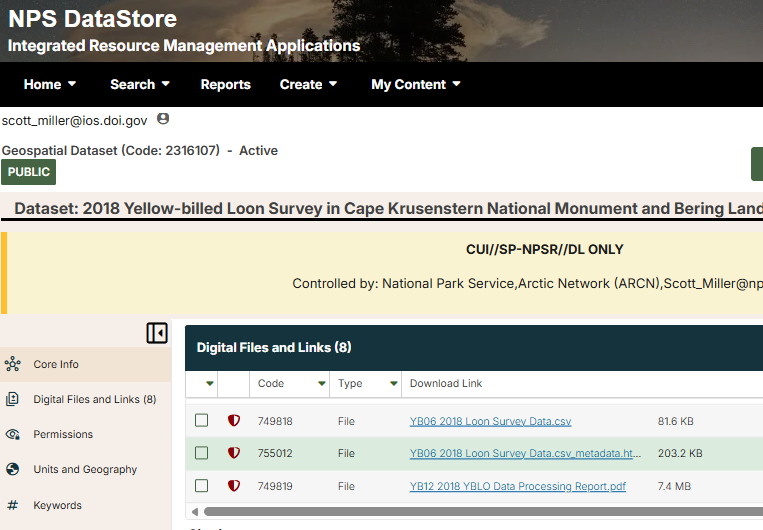
\includegraphics[width=5.41667in,height=\textheight,keepaspectratio]{images/clipboard-3271303711.png}

Figure 2. Example of an annual loon survey deliverables archived as a
Geospatial Dataset in NPS Data Store. Annual survey files (see
Deliverables Schedule and Figure 1.) are archived as private,
NPS-Internal References in Data Store.

\subsection{Certified dataset
publication}\label{certified-dataset-publication}

Certified dataset. This dataset is cumulative. Each year's data is
appended to the loons monitoring master database and then the
\texttt{Dataset\_Certified} query exported to a CSV file and the
\href{https://irma.nps.gov/DataStore/Reference/Profile/2316912}{Certified
Dataset Reference} in Data Store is versioned with the new file.

\section{Review and revise the Standard Operating
Procedures}\label{review-and-revise-the-standard-operating-procedures}

If any methodologies have improved or changed significantly then update
the
\href{https://irma.nps.gov/DataStore/Reference/Profile/2216938}{SOPs}.

\bookmarksetup{startatroot}

\chapter*{References}\label{references}
\addcontentsline{toc}{chapter}{References}

\markboth{References}{References}

\phantomsection\label{refs}
\begin{CSLReferences}{1}{0}
\bibitem[\citeproctext]{ref-flamme2018}
Flamme, J. H. Schmidt, M., and S. D. Miller. 2018. {``Yellow-Billed Loon
Monitoring Protocol for the Arctic Network: Protocol Narrative Version
1.0.''} Natural Resource Report NPS/ARCN/NRR---2018/1738. Fort Collins,
Colorado: National Park Service.
\url{https://irma.nps.gov/DataStore/Reference/Profile/2256435}.

\bibitem[\citeproctext]{ref-koelsch2019}
Koelsch, J. 2019. {``To: Wald EJ. Re: Handling of Protected Natural
Resource Data - BELA.''}
\url{https://irma.nps.gov/DataStore/Reference/Profile/2263477}.

\bibitem[\citeproctext]{ref-wickham2014tidydata}
Wickham, Hadley. 2014. {``Tidy Data.''} \emph{Journal of Statistical
Software} 59 (10): 1--23. \url{https://doi.org/10.18637/jss.v059.i10}.

\end{CSLReferences}




\end{document}
